Di seguito viene riportata la tabella contenente le ore totali rendicontate che ogni componente del gruppo ha dedicato per lo sviluppo del progetto.

\begin{table}[h]
	\centering
	\begin{tabular}{|l|c|c|c|c|c|c|c|}
		\toprule
		\textbf{Cognome e Nome} & \multicolumn{6}{c}{\textbf{Ore per ruolo}} & \textbf{Ore Totali} \\
		& \textbf{Re} & \textbf{Am} & \textbf{An} & \textbf{Pt} & \textbf{Pr} & \textbf{Ve} & \\
		
		\midrule
		Agostinetto Matteo & 5 & 4 & & 26 & 35 & 35 & 105 \\
		Burlin Valerio & & 4 & 17 & 28 & 32 & 24 & 105 \\ 
		Carraro Nicola & 4 & & & 32 & 33 & 36 & 105 \\
		Crespan Emanuele & & & 4 & 27 & 23 & 31 & 85 \\
		Ros Fabio & & 8 & & 36 & 33 & 28 & 105 \\
		Suierica Bogdan & 4 & & 10 & 31 & 31 & 29 & 105 \\
		
		\bottomrule
	\end{tabular}
	\caption{Ore rendicontate a componente per ruolo, consuntivo finale}
\end{table}

\noindent Tale rendicontazione deriva, oltre che dagli strumenti di collaborazione predisposti dall'\textit{Amministratore di Progetto} per lo svolgimento e monitoraggio delle attività dei membri del gruppo, dai due verbali \textit{} e \textit{} risultanti da problemi interni al gruppo, dovuti a scarso impegno e non rispetto delle \textit{Norme di Progetto v4.0.0}, in particolare la totale assenza ed irreperibilità di un componente, citato in tali verbali. Oltre a ciò, la diminuzione di ore rendicontate a tale componente è dovuta anche ad un maggiore carico di studio personale delle tecnologie per effettuare i test di unità del sistema, che ne hanno ridotto l'impegno effettivo nella realizzazione del progetto. 

\noindent La tabella seguente riporta le differenze dell'incidenza oraria dei ruoli di progetto tra quanto pianificato e quanto realmente impiegato. I valori negativi nella tabella indicano un monte ore maggiore di quello preventivato, i valori positivi una diminuzione di ore.

\begin{table}[h]
	\centering
	\begin{tabular}{|l|c|c|c|}
		\toprule
		\textbf{Ruolo} & \textbf{Ore preventivate} & \textbf{Ore impiegate} & \textbf{Differenza} \\
		
		\midrule
		Responsabile di Progetto & 17 & 13 & +4 \\
		Amministratore di Progetto & 17 & 16 & +1 \\ 
		Analista & 28 & 31 -3 & \\
		Progettista & 189 & 180 & +9 \\
		Programmatore & 190 & 187 & +3 \\
		Verificatore & 183 & 189 & -6 \\
		\midrule
		\textbf{Totale} & 624 & 616 & +8 \\
		
		\bottomrule
	\end{tabular}
	\caption{Costo rendicontato per ruolo, consuntivo finale}
\end{table}

\newpage
\noindent Il seguente grafico mostra la differenza dell'impiego orario dei vari ruoli tra quanto pianificato e quanto impiegato.

\begin{figure}[h]
	\centering
	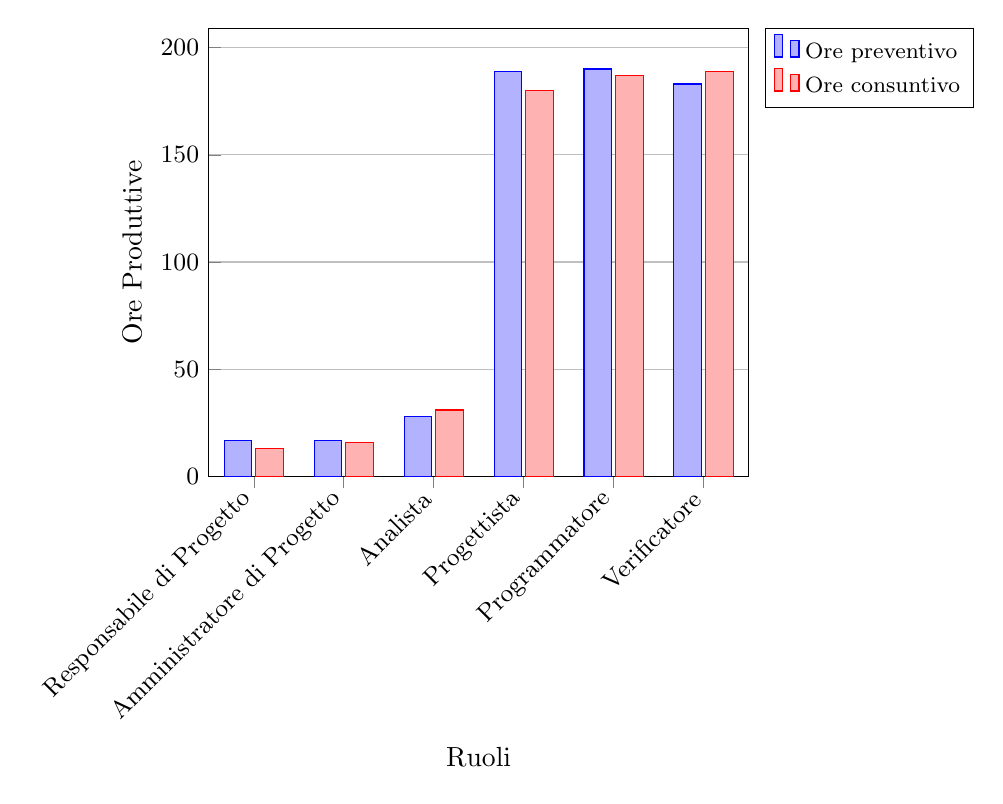
\begin{tikzpicture}
	\begin{axis}[
	ybar,
	tick label style={font=\small},
	tickpos=left,
	xlabel = {Ruoli},
	ylabel = {Ore Produttive},
	xticklabels={Responsabile di Progetto, Amministratore di Progetto, Analista, Progettista, Programmatore, Verificatore}, 
	xtick={1,2,3,4,5,6},
	x tick label style = {rotate=45,anchor=east},
	ymin=0,
	ymajorgrids = true,
	legend pos = outer north east,
	legend style = {nodes=right,font=\footnotesize},
	]
	\addplot +[bar shift=-.2cm] plot coordinates {(1, 17) (2, 17) (3, 28) (4, 189) (5, 190) (6, 183)};
	
	\addplot +[bar shift=.2cm] plot coordinates {(1, 13) (2, 16) (3, 31) (4, 180) (5, 187) (6, 189)};
	\legend{\strut Ore preventivo, \strut Ore consuntivo}
	\end{axis}
	\end{tikzpicture}
	\caption{Consuntivo orario rendicontato per ruoli}
\end{figure}

\noindent Di seguito viene riportato il consuntivo finale del progetto \PROGETTO{}. La tabella riporta i costi totali sostenuti dal gruppo per ogni periodo. Si fa notare che nella tabella sono riportati solo i periodi che sono effettivamente a carico del Committente.

\begin{table}[h]
	\centering
	\begin{tabular}{|l|c|c|c|c|c|c|c|}
		\toprule
		\textbf{Periodo} & \textbf{Tipo} & \textbf{Costo} \\
		
		\midrule
		Progettazione Architetturale & consuntivo & \textcolor{green}{3456} \\
		Progettazione di Dettaglio e Codifica & consuntivo & \textcolor{green}{5079} \\ 
		Verifica e Validazione & preventivo & \textcolor{green}{2460} \\
		
		\midrule
		Costo Totale & & \textcolor{green}{10995} \\
				
		\bottomrule
	\end{tabular}
	\caption{Consuntivo finale}
\end{table}

\noindent In totale il gruppo ha risparmiato \textbf{398} dovuti alla riprogrammazione effettuata durante il periodo di \textit{Progettazione di Dettaglio e Codifica} ed alla carenza di ore dedicate al progetto da parte di un componente del gruppo, come citato sopra. Questo è stato uno dei fattori della riprogrammazione effettuata, comunque il modo di lavoro appreso e utilizzato da parte degli altri componenti del gruppo ha comunque permesso di consegnare il progetto completo nei suoi requisiti obbligatori, tralasciando molti requisiti opzionali e desiderabili.